\documentclass[12pt,DIV14,BCOR10mm,a4paper,parskip=half-,headsepline,headinclude,english,ngerman,bibliography=totocnumbered]{scrreprt}

\usepackage{hshhelper_base}

%%%%%%%%%%%%%%%%%%%%%%%%%%%%%%%%%%%%%%%%%%%%%%%%%%%%%%%%%%%%%%%%%%%%%%%%%%
\begin{document}    % hier gehts los
  \thispagestyle{empty} % Titelseite

\includegraphics[width=0.2\textwidth]{Wortmarke_WI_schwarz}

   {  ~ \sffamily
  \vfill
  {\Huge\bfseries Bedrohungsanalyse}
  \bigskip

  {\Large
  Dennis Grabowski, Julius Zint, Philip Matesanz, Torben Voltmer \\[2ex]
  Masterprojekt \enquote{Entwicklung und Analyse einer sicheren \\Web-Anwendung} \\
  Wintersemester 18/19
 \\[5ex]
   \today }
}
 \vfill

  ~ \hfill
  
\includegraphics[height=0.3\paperheight]{H_WI_Pantone1665}

\vspace*{-3cm}

\tableofcontents  % Inhaltsverzeichnis

\chapter{Zur Analyse verwendeten Methoden}
\section{Dataflow Diagram}

Das folgende \gls{dfd} wurde mithilfe des Programms \enquote{OWASP Threat Dragon} \autocite{OWASP.ThreatDragon} erstellt.
Dieses Programm erlaubt leider keine Einfärbung in grün zur Kennzeichnung vertrauenswürdiger Prozesse oder Datenflüsse.
Alle schwarz gekennzeichneten Elemente sind daher als vertrauenswürdig zu betrachten.

\begin{figure}[htbp]
  \hspace*{-2.5cm}
  \label{overview-dfd-pic}
  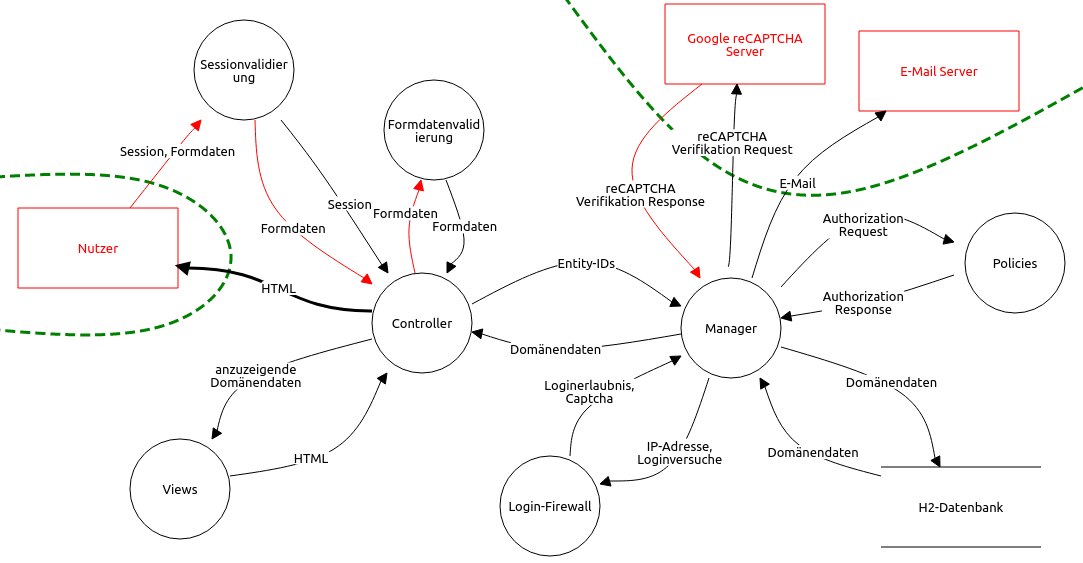
\includegraphics[width=1.25\linewidth]{resources/overview-dfd.jpg}
  \caption{Gesamtübersicht des Datenflusses in unserer Applikation}
\end{figure}

\subsection{Layered Entrypoints}

\begin{enumerate}
  \item HTTP (Port 80)
  \begin{enumerate}
    \item \texttt{HomeController}
    \begin{enumerate}
      \item GET - \texttt{/}
    \end{enumerate}

 \item \texttt{LoginController}
    \begin{enumerate}
     \item \texttt{/login}
      \begin{enumerate}
        \item GET - \texttt{showLoginForm()}
        \item POST - \texttt{login(username, password, recaptcha)}
      \end{enumerate}
      \item \texttt{/logout}
      \begin{enumerate}
        \item POST - \texttt{logout()}
      \end{enumerate}
      \item \texttt{/changePasswordAfterReset}
      \begin{enumerate}
        \item GET - \texttt{showChangePasswordAfterResetForm}
        \item POST - \texttt{changePasswordAfterReset(username, currentPassword, password, passwordRepeat, recaptcha)}
      \end{enumerate}
    \end{enumerate}
    \item \texttt{UserController}
    \begin{enumerate}
      \item \texttt{/users}
      \begin{enumerate}
        \item GET - \texttt{showUsers()}
      \end{enumerate}
      \item \texttt{/users/create}
      \begin{enumerate}
        \item GET - \texttt{showCreateUserForm()}
        \item POST - \texttt{createUser(username, email)}
      \end{enumerate}
      \item \texttt{/users/delete}
      \begin{enumerate}
        \item POST - \texttt{deleteUser(userId)}
      \end{enumerate}
      \item \texttt{/resetpassword}
      \begin{enumerate}
        \item GET - \texttt{showResetUserPasswordForm}
        \item POST - \texttt{resetUserPassword(username)}
      \end{enumerate}
      \item \texttt{/sessions}
      \begin{enumerate}
        \item GET - \texttt{showActiveUserSessions()}
      \end{enumerate}
      \item \texttt{/sessions/delete}
      \begin{enumerate}
        \item POST - \texttt{deleteUserSession()}
      \end{enumerate}
    \end{enumerate}

    \item \texttt{GroupController}
    \begin{enumerate}
      \item \texttt{/user/groups}
      \begin{enumerate}
        \item GET - \texttt{showOwnGroups}
      \end{enumerate}
      \item \texttt{/groups}
      \begin{enumerate}
        \item GET - \texttt{showAllGroups}
      \end{enumerate}
      \item \texttt{/groups/create}
      \begin{enumerate}
        \item GET - \texttt{showCreateGroupForm}
        \item POST - \texttt{createGroup(groupname)}
      \end{enumerate}
      \item \texttt{/groups/:groupId}
      \begin{enumerate}
        \item GET - \texttt{showGroup(groupId)}
      \end{enumerate}
      \item \texttt{/groups/:groupId/members/remove}
      \begin{enumerate}
        \item POST - \texttt{removeGroupMember(groupId, userId)}
      \end{enumerate}
      \item \texttt{/groups/:groupId/members/add}
      \begin{enumerate}
        \item POST - \texttt{addGroupMember(groupId, userId)}
      \end{enumerate}
      \item \texttt{/groups/:groupId/delete}
      \begin{enumerate}
        \item POST - \texttt{deleteGroup(groupId)}
      \end{enumerate}
    \end{enumerate}
  \end{enumerate}
  \item SMTP (Port 587)
  \begin{enumerate}
    \item Versand der E-Mail für den Passwort-Reset (username, email, tempPassword)
  \end{enumerate}
\end{enumerate}

\chapter{Bedrohungen}
\section{Gefundene Bedrohungen}

\subsection{Globale Bedrohungen}

\begin{itemize}
  \item \textbf{Spoofing des Servers}
  \begin{itemize}
  \item Zweck: 
  	\begin{itemize}  
  		\item Ausspähen von Anmeldedaten der Benutzer
  		\item Ausspähen von Dateien, die ein Benutzer bei HshHelper hochladen möchte
  	\end{itemize}
  \item Möglichkeiten: \textcolor{red}{IP-Spoofing, DNS manipulieren,...}
  	\begin{itemize}  
  		\item Ausspähen von Anmeldedaten der Benutzer
  		\item Ausspähen von Dateien, die ein Benutzer bei HshHelper hochladen möchte
  	\end{itemize}
  \item Risiko: Mittelmäßig
  \item Gegenmaßnahmen: Authentifizierung des HshHelper Servers durch Zertifikate (HTTPS mit HSTS)
  \end{itemize}

  \item \textbf{Eavesdropping}
  \begin{itemize}
  \item Zweck: 
  	\begin{itemize}  
  		\item Ausspähen von Anmeldedaten der Benutzer
  		\item Ausspähen von  \textcolor{red}{eigentlich allen Daten}
  		\item Ausspähen von Dateien, die ein Benutzer bei HshHelper hochlädt
  		\item Ausspähen von Dateien, die ein Benutzer bei HshHelper runterlädt
  	\end{itemize}
  \item Möglichkeiten: Man-in-the-Middle-Angriff
  \item Risiko: Mittelmäßig
  \item Gegenmaßnahmen: Verschlüsselung durch HTTPS mit HSTS oder SecureCookie
  \end{itemize}

  \item \textbf{Replayattacken}
  \begin{itemize}
  \item Zweck:
  \item Möglichkeiten:
  \item Risiko: Mittelmäßig
  \item Gegenmaßnahmen: HTTPS / CSRF-Token
  \end{itemize}

  \item \textbf{Tampering}
  \begin{itemize}
  \item Zweck:
  \item Möglichkeiten:
  \item Risiko: Mittelmäßig
  \item Gegenmaßnahmen: HTTPS
  \end{itemize}

  \item \textbf{Verwendung eines gefälschten,von einer anerkannten Zertifizierungsstelle signierten Zertifikates}%Ungültig ausgestelltes Zertifikat (Türkischer Geheimdienst)
  \begin{itemize}
  \item Zweck: 
  	\begin{itemize}
  		\item Spoofing des Servers
  		\item Man-in-the-Middle-Angriffe
   \end{itemize}
  \item Möglichkeiten: Kontrolliert man eine anerkannten Zertifizierungsstelle, können gefälschte Zertifikate für die HshHelper Domain ausgestellt werden. Für HshHelper Benutzer ist das nicht sofort einsehbar.
  \item Risiko: Gering
  \item Gegenmaßnahmen: HTTP Public Key Pinning (HPKP)
  \end{itemize}


  \item \textbf{XSS (Cross Site Scripting)}
  \begin{itemize}
  \item Zweck: Ausführung von JavaScript im HshHelper Kontext eines Benutzers
  \item Möglichkeiten:
  	\begin{itemize}
          \item Skript einbetten in Benutzername bei der Erstellung eines Nutzers
          \item Skript einbetten in Gruppennamen bei der Erstellung einer Gruppe
      \end{itemize}
  \item Risiko: Hoch
  \item Gegenmaßnahmen:
	\begin{itemize}
		\item Content Security Policy (CSP) des Browsers aktivieren. \textcolor{red}{Alte Browser bzw Browser die CSP nicht können aussperren} %TODO: Das ist nicht implementiert und vllt auch garnicht so einfach. Ggf einfach in Assumptions aufnehmen, dass nur Browser verwendet werden, die CSP unterstützen
		\item Ausgabecodierung
	\end{itemize}
  \end{itemize}
      Eingabevalidierung (Kleinbuchstaben und Zahlen, valide E-Mail-Adressen)

  \item \textbf{SQL Injection}
  \begin{itemize}
  \item Zweck: Ungültige Manipulation von Datenbankeinträgen
  \item Möglichkeiten: Lesen und schreiben von Datenbankinhalten
  \item Risiko: Hoch
  \item Gegenmaßnahmen:
  \begin{itemize}
    \item Die H2 Einstellung \texttt{ALLOW\_LITERALS=NONE} verwenden
    \item Nur PreparedStatements benutzen
    \item Eingabevalidierung
  \end{itemize}
  \end{itemize}

  \item \textbf{CSRF (Cross-Site-Request-Forgery)}
  \begin{itemize}
  \item Zweck:
  \item Möglichkeiten:
  \begin{itemize}
          \item Einen fremden Benutzer ausloggen
          \item Einem Administrator einen Request unterjubeln, durch welchen er einen Nutzer erstellt
  \end{itemize}
  \item Risiko: Hoch
  \item Gegenmaßnahmen: CSRF-Tokens bei Requests checken
  \end{itemize}

  \item \textbf{Session fälschen (eine bestimmte oder irgendeine?)}
  \begin{itemize}
  \item Zweck: Client spoofen
  \item Möglichkeiten:
  \item Risiko: Hoch
  \item Gegenmaßnahmen: Signieren des Cookies durch PrivateKey und Verwendung von UUID, Bindung an IP-Adresse, Begrenzung der Lebenszeiten(?)
  \end{itemize}

  \item \textbf{Abstreitbarkeit illegaler Handlungen}
  \begin{itemize}
  \item Zweck:
  \item Möglichkeiten: Eintragen illegaler Namen bei Benutzernamen oder Gruppenmane
  \item Risiko: Gering
  \item Gegenmaßnahmen: Logging von IP + Zeit, Action, User
  \end{itemize}

  \item \textbf{Nutzer kann eine ihm unerlaubte Operation durchführen}
  \begin{itemize}
  \item Zweck: Beispielsweise um einen Denial-of-Service-Angriff auf einen Nutzer durchzuführen
  \item Möglichkeiten: Beispielsweise Nutzer löscht andere Nutzer
  \item Risiko: Mittelmäßig - Hoch
  \item Gegenmaßnahmen: Authorization erzwingen und prüfen bei jeder Operation
  \end{itemize}

  \item \textcolor{red}{Captcha lösen lassen von Indern?}
  \item \textcolor{red}{Elevation of privilege -> Frage an Peine. ?}
\end{itemize}

\subsection{HTTP-Endpoint-spezifische Bedrohungen}

\subsubsection{Mögliche Angriffe auf den Loginprozess}

\begin{itemize}
  \item \textbf{Überlanges PW beim Login eingeben}
  \begin{itemize}
  \item Zweck: Zum DDOSn der Applikation
  \item Möglichkeiten: Durch Eingabe eines überlangen Passworts braucht der Hashing-Algorithmus sehr lange
  \item Risiko: Gering
  \item Gegenmaßnahmen:
  \begin{itemize}
  \item Passwort-Länge mittels Eingabevalidierung beschränken
  \item Verwendung von bcrypt (lässt nur 72 Zeichen lange Passwörter zu, Lauzeit ist für alle Längen von Eingaben konstant)
  \end{itemize}
\end{itemize}

  \item \textbf{Timing-Angriff auf Loginverhalten}
  \begin{itemize}
  \item Zweck: Herausfinden, ob ein Benutzer mit einem bestimmten Username existiert
  \item Möglichkeiten: Durch Messen der Antwortszeiten des Servers können Rückschlüsse darüber gezogen werden, welcher Code ausgeführt wurde (zB Hashing/DB-Zugriff)
  \item Risiko: Mittelmäßig-Hoch
  \item Gegenmaßnahmen: Loginprozess für jeden Fall gleich ablaufen lassen
  \end{itemize}

  \item \textbf{Online Brute-forcing}
  \begin{itemize}
  \item Zweck: Zum Knacken eines Benutzeraccounts
  \item Möglichkeiten: Beispielsweise durch Wörterbuchattacken
  \item Risiko: Hoch
  \item Gegenmaßnahmen:
  \begin{itemize}
      \item Captcha Mode = Login nur möglich, wenn Captcha gelöst wird.
      \item Accounts müssen nach x falschen Logins, einen Captcha lösen, sowie IP-Adressen sperren nach Y falschen Logins
      \item Schwache Passworter verbieten
      \item \textcolor{red}{Zwei-Factor-Authentication} % TODO: Ist nicht implementiert und ggf auch nicht mal eben so gemacht
    \end{itemize}
  \end{itemize}
\end{itemize}

\subsubsection{Mögliche Angriffe auf den \enquote{Passwort zurücksetzen lassen}-Prozess}

\begin{itemize}
  \item \textbf{Nutzer permanent aus der Applikation ausschliessen}
  \begin{itemize}
  \item Zweck: Denial-of-Service-Angriff auf einen individuellen Nutzer
  \item Möglichkeiten: Wiederholtes Absenden des Request mit richtigen Nutzernamen generiert bei jedem Request ein neues temporäres Passwort. Selbst wenn der Benutzer das temporäre Passwort ändert, wird er es nicht schaffen sich anzumelden, da dann bereits die Generierung ein neues temporäres Passwort vom Angreifer erzwungen wurde.
  \item Risiko: Mittel
  \item Gegenmaßnahmen:
  \begin{itemize}
  \item Einbau eines Captchas
  \item Dem Benutzer einen Link schicken, der geöffnet werden muss, um den \enquote{Passwort ändern}-Prozess anzustoßen. Der Link muss einen geheimen Token beinhalten, der nur HshHelper und dem Empfänger der E-Mail bekannt ist. Das temporäre Passwort wird erst generiert, sobald auf den Link geklickt wird
  \end{itemize}
\end{itemize}

  \item \textbf{Timing-Angriff auf Verhalten des Requests}
  \begin{itemize}
  \item Zweck: Herausfinden, ob ein Benutzer mit einem bestimmten Username existiert
  \item Möglichkeiten: Durch Messen der Antwortszeiten des Servers können Rückschlüsse darüber gezogen werden, welcher Code ausgeführt wurde (E-Mail-Versand)
  \item Risiko: Mittelmäßig-Hoch
  \item Gegenmaßnahmen:
  \begin{itemize}
    \item \enquote{Passwort zurücksetzen lassen}-Prozess in konstanter Länge ablaufen lassen \textcolor{red}{Ggf. E-Mail an fakeaddresse beim falschen Nutzername}
    \item E-Mail-Versand asynchron durchführen
    \end{itemize}
  \end{itemize}

  \item \textbf{E-Mail Postfach des Nutzers spammen}
  \begin{itemize}
  \item Zweck: Verbrauch der vorhandenen Resourcen seines E-Mail-Kontos
  \item Möglichkeiten: Wiederholtes Absenden des Forms durch Angabe seines Nutzernamens
  \item Risiko: Hoch
  \item Gegenmaßnahmen: Nutzer muss Captcha lösen bevor Prozess angestoßen werden darf
  \end{itemize}
\end{itemize}

\subsubsection{Mögliche Angriffe auf den \enquote{Passwort ändern}-Prozess}

% This is subject to change if we implement the link-based mitigation
Da dieser Prozess dem Loginprozess gleich ist, treten hier die selben Lücken auf.
Um das Dokument kurz zu halten, listen wir diese nicht nochmal auf.

\section{Ignorierte Bedrohungen}

Die hier aufgelisteten Bedrohungen werden ignoriert, da wir im Rahmen des Projekts definiert haben, dass nur Angriffe über den HTTP-Vektor betrachtet werden.

\subsubsection{DDOS}
\begin{itemize}

  \item \textbf{DDOS (Out of scope)}
  \begin{itemize}
  \item Zweck: standard Zweck
  \item Möglichkeiten: standard means
  \item Risiko:
  \item Gegenmaßnahmen: None, or standard IDS
  \end{itemize}
\end{itemize}


\subsubsection{Mögliche Angriffe beim Versand der Passwort-Reset-E-Mail}

\begin{itemize}
  \item E-Mailversand abhören
    \begin{itemize}
    \item Zweck:
    \item Möglichkeiten:
    \item Risiko:
    \item Gegenmaßnahmen: SMTPS (Two-Faktor-Authentisierung)?
    \end{itemize}

  \item Serverresourcen aufbrauchen
    \begin{itemize}
    \item Zweck: Denial-of-Service auf den Server durch Verschwenden seiner Resourcen
    \item Möglichkeiten: Angreifer nutzt "Passwort zurücksetzen"-Formular als Angriffsvektor zum Versenden vieler Mails
    \item Risiko: High
    \item Gegenmaßnahmen: E-Mail nicht beliebig oft senden lassen
    \end{itemize}

  \item Server zum Warten beim E-Mail-Versand zwingen
    \begin{itemize}
    \item Zweck: Denial-of-Service auf den Server
    \item Möglichkeiten: Angreifer spoofed IP-Adresse des E-Mail-Servers und zwingt Server zum Warten, beispielsweise durch Delay seiner Response
    \item Risiko: Gering-Mittel
    \item Gegenmaßnahmen: SMTPS, ggf. Sender Policy Framework
    \end{itemize}
\end{itemize}

\textcolor{red}{
Beispielsweise via Betriebssystem, physikalischer Zugriff auf der Maschine oder HTTPS?
Oder welche, für die es keine Motivation gibt, ggf. Repudiations
}

\section{HTTP Header}

In der folgenden Liste werden verschiedene sicherheitsrelevante \enquote{HTTP Headers} beschrieben, die uns helfen, einige der Gegenmaßnahmen zu realisieren.
Diese Werte werden empfohlen, um die \enquote{maximale} Sicherheit zu garantieren.
Entnommen haben wir diese Empfehlungen verschiedenen Seiten, darunter der \enquote{Mozilla's Enterprise Information Security}-Blog \autocite{Mozilla.SecureHeaders} und das \enquote{OWASP Secure Headers Project} \autocite{OWASP.SecureHeaders}, die wir beide als vertrauenswürdig betrachten.

\subsection{Referrer-Policy}
\begin{sloppypar}
\texttt{Referrer-Policy: origin-when-cross-origin, strict-origin-when-cross-origin}
\end{sloppypar}
Mit diesem Header kann gesteuert werden, welche Informationen als \enquote{Referrer} an die nächste besuchte Seite weitergegeben werden. \texttt{strict-origin-when-cross-origin} sorgt dafür, dass innerhalb der Seite die vollständige URL weitergegeben wird. Beim Besuchen einer anderen Seite wird nur die Domain weitergegeben. Wird dabei jedoch von HTTPS auf HTTP gewechselt, ist das Weitergeben jeder Information untersagt.

\textcolor{red}{
TODO: Explizit in Play nur strict-origin-when-cross-origin machen
}
\subsection{X-Frame-Options}
\begin{sloppypar}
\texttt{X-Frame-Options: DENY}
\end{sloppypar}
Um zu verhindern, dass unsere Seite in einem \texttt{<frame>}, \texttt{<iframe>} oder \texttt{<object>} Element auf einer anderen Seite eingebettet wird, kann der Header \texttt{X-Frame-Options} verwendet werden. So können \enquote{Clickjacking} sowie \texttt{<iframe>}-basierte CSRF-Angriffe verhindert werden.

\subsection{X-XSS-Protection}
\begin{sloppypar}
\texttt{X-XSS-Protection: 1; mode=block}
\end{sloppypar}
Durch den Header \texttt{X-XSS-Protection} wird der Browser angewiesen, eine XSS Erkennung zu versuchen. Dieses Feature ist für älteren Browser interessant, die noch kein CSP implementieren. Durch den Modus \enquote{block} wird das Laden der Seite abgebrochen, sobald ein XSS Versuch erkannt wird.

\subsection{X-Content-Type-Options}
\begin{sloppypar}
\texttt{X-Content-Type-Options: nosniff}
\end{sloppypar}
Mit diesem Header wird dem Browser verboten, \enquote{MIME sniffing}\footnote{Beim \enquote{MIME sniffing} versucht der Browser den richtigen MIME Type durch Betrachtung des Inhalts zu erraten, wenn er annimmt, dass der im \texttt{Content-Type} übermittelte Wert nicht korrekt ist.} zu betreiben. Er wird gezwungen den MIME Typ zu verwenden, der im \texttt{Content-Type} Header angegeben wurde.

\subsection{Content-Security-Policy}
\begin{sloppypar}
\texttt{Content-Security-Policy: default-src 'self'; script-src https://www.google.com/recaptcha/ https://www.gstatic.com/recaptcha/; frame-src https://www.google.com/recaptcha/}
\end{sloppypar}
Innerhalb diesem Header ist es möglich Richtlinien zu definieren, die den Zugriff auf verschiedene Resourcen kontrollieren.
Dadurch kann verhindert werden, dass JavaScript nicht von jeder URL geladen und ausgeführt werden darf, von welchen Quellen Bilder geladen werden dürfen, oder welches CSS eingebunden werden darf.
Dieser Header ist dem \enquote{X-XSS-Protection}-Header vorzuziehen.

\subsection{X-Permitted-Cross-Domain-Policies}
\begin{sloppypar}
\texttt{X-Permitted-Cross-Domain-Policies: master-only}
\end{sloppypar}

\printbibliography

% Can be used to add a list of acronyms with their description
%\glsaddall
%\deftranslation{to=German}{Acronyms}{Abkürzungsverzeichnis}
%\deftranslation{to=German}{Glossary}{Glossar}
\printacronyms[title=Abkürzungsverzeichnis,toctitle=Abkürzungsverzeichnis]
\printglossary[type=main]

%\addcontentsline{toc}{chapter}{\listfigurename}
\listoffigures      % Abbildungsverzeichnis

%s\addcontentsline{toc}{chapter}{\listtablename}
% \listoftables       % Tabellenverzeichnis

\end{document}
